\documentclass[12pt,twoside,a4paper]{report}

\usepackage[inner=35mm, outer=24mm, top=24mm, bottom=24mm]{geometry}
\usepackage[parfill]{parskip}

\usepackage{hyperref}
\usepackage[title]{appendix}

\usepackage{float}
\usepackage{graphicx}
\graphicspath{ {images/} }
\usepackage{subcaption}

\usepackage{xcolor}
\usepackage{listings}

\definecolor{mGray}{rgb}{0.5,0.5,0.5}
\definecolor{backgroundColour}{rgb}{1,1,1}

\lstdefinestyle{CStyle}
{
    backgroundcolor=\color{backgroundColour},   
    commentstyle=\color{mGray},
    keywordstyle=\color{mGray},
    numberstyle=\tiny\color{mGray},
    stringstyle=\color{mGray},
    basicstyle=\footnotesize,
    breakatwhitespace=false,         
    breaklines=true,                 
    captionpos=b,                    
    keepspaces=true,                 
    numbers=left,                    
    numbersep=5pt,                  
    showspaces=false,                
    showstringspaces=false,
    showtabs=false,                  
    tabsize=2,
    language=C
}

\usepackage{lipsum}
\usepackage{draftwatermark}
\SetWatermarkScale{8} 

\begin{document}
    
    \begin{titlepage}
    \begin{center}
        \Huge
        Electronics and Computer Science
        \\Faculty of Physical and Applied Sciences
        \\University of Southampton
        \Large
        \\[4cm]Author: Lewis Smith
        \\[1cm]\today
        \\[2cm]Low Power Hardware Accelerated Internet of Things Cryptography
        \\[4cm]Project Supervisor: Mark Zwolinski
        \\Second Examiner:
        \\[4cm]A project report submitted for the award of MEng Electronic Systems with Computer Systems
        
    \end{center}
    \end{titlepage}
    \thispagestyle{empty}
    \cleardoublepage
    
    \begin{abstract}
    
    \addcontentsline{toc}{chapter}{Abstract}    
    \lipsum[1-2]
    
    \end{abstract}
    
    \tableofcontents
    \addcontentsline{toc}{chapter}{Contents}
    
    \chapter*{Acknowledgements}
    \addcontentsline{toc}{chapter}{Acknowledgements}
    
    \chapter{Introduction}
    \label{chapter:intro}
    As the speed and global reach of the internet has expanded over the years the number of devices connected to it has rapidly increased. These devices are no longer just the servers and the PC's connected to them, they now include consumer devices like smartphones, tablets, and games consoles. However, even more recently the idea of connecting the internet to various `dumb' appliances like: simple light switches; kettles; fridges and many more; to make them `smart' devices that can be controlled through small embedded processors has emerged. The idea of connecting such devices to internet has been dubbed `Internet of Things' or `IoT' and has the aim to make our lives simpler. The `IoT' concept is also being explored for more industrial applications such as: automated factories; and city electrical grids; and even a network of self-driving cars\cite{Hegde} but this is far more advanced than the basic `smart' home.
    
    Due to the wide range of products that a connected IoT device can be applied to improve the efficiency and/or usefulness, it has been predicted that billions of devices will be in use by 2020\cite{Evans2011}. This also means that the complexity of the devices varies greatly. The one thing that all of these devices have in common though is that they need to be secure as they communicate sensitive and private data through an open channel on the internet between the user and the device. To keep the potential adversaries from accessing the data and possibly controlling numerous connected devices, maliciously or not, an encryption algorithm can be used.
    
    \textcolor{orange}{POSSIBLY CHANGE/IMPROVE BELOW}      
        
    There are many encryption algorithms that perform this function and most can be implemented in both software and dedicated hardware such as an Application Specific Integrated Circuit (ASIC) or a Field Programmable Gate Array (FPGA). As a majority of IoT devices are implemented on small embedded processors which have limited resources, the hardware option might possibly be a better solution for IoT devices. However, due to the fact that most IoT devices are always on, and likely battery powered, power consumption is a very important factor when considering options for adding hardware accelerated encryption and for battery powered devices it is often more critical than the actual encryption.
    
    The goals of this project are to explore various encryption algorithms and compare their performance based on data throughput, accuracy, security and power consumption when implemented in software and hardware. To evaluate these parameters the same algorithms can be coded in C or C++ for the software versions and a Hardware Development Language (HDL) such as System Verilog can be first simulated in ModelSim, before programming a FPGA for the hardware version. These comparisons can then be used to match the algorithms to the appropriate IoT device as they all have different requirements for relative security level and power consumption, as for example a light switch does not necessarily need to be protected from the same level of attack as a set of digital locks or private data storage. In order for the hardware to work with IoT devices it will also need a communication protocol like $I^2 C$ or SPI to work with embedded processors, and possibly Ethernet or WiFi to act as the gateway to internet for the device. Some of these protocols are available on FPGA development boards but can be implemented in System Verilog code.
    
    \chapter{Background Research \& Literature}
    \label{section:BACK}
    
    \section{Internet of Things}
    \label{section:IoT}
    
    \textcolor{red}{CHANGE/IMPROVE BELOW}
    
    As mentioned in \autoref{chapter:intro} there are many IoT devices that require varying levels of security and have to be protected against different of attacks, like side channel attacks. The purpose of this subsection is to discover what these devices are and what properties are required in the encryption algorithm in terms of throughput, power or energy consumption, software or hardware restrictions and security. Due to IoT devices having limited resources \cite{Juels2005} suggests that 2000 Gate Equivalents in hardware is the maximum size for most embedded platforms but even that might be to big for devices like RFID tags. Power consumption should also be kept to as little as possible but \cite{David2011} outlines a limit of tens of micro Watts ($\mu W$) for RFID tags.
    
    \section{Cryptography}
    \label{section:crypt}
    
    \textcolor{orange}{POSSIBLY CHANGE/IMPROVE BELOW}
    
    After evaluating the conditions required to provide the appropriate level of security  in \autoref{section:IoT} this subsection explores the cryptographic principles and algorithms available that satisfy those conditions. The primary objective of cryptography is to convert, or encrypt, a readable message known as plaintext into an unreadable form, ciphertext, so that adversaries cannot read the contents, but over the years the scope of cryptography has widened. Throughout history encryption has been has been used allow people and groups to exchange secret messages, especially in times of war. Since the early transposition and substitution ciphers, where each character in a message are rearranged and replaced by others a certain number further down the alphabet respectively, encryption has evolved to include techniques for identity authentication, integrity checks and much more\textcolor{red}{[insert reference]}. Cryptography is therefore the study of encryption and other techniques, including identity authentication and integrity checks. Its counterpart: the study of breaking the encryption to find the original message, is known as cryptanalysis\cite{AlfredJ.Menezes1996}. Eventually, for most encryption techniques a weakness is found, and subsequently exploited, so more complex techniques are conceived and with the invention of computers the complexity of the algorithms has increased greatly. However, the computer power is also available for cryptanalysis so the cycle of continuous improvement of the algorithms hasn't stopped.
    
    In cryptography there are two main concepts that the algorithms are based on: symmetric and asymmetric keys\textcolor{red}{[insert reference]}. In asymmetric key cryptography a unique key is used to encrypt data and different, but a related key, is used to decrypt it. The relationship between the two keys is often defined by maths problem that is very difficult to solve which is the basis of the encryption\textcolor{red}{[insert reference]}. On the other hand, symmetric key cryptography uses the same key for both encryption and decryption, hence symmetric, with the security usually provided by a combination of simple logic operations\textcolor{red}{[insert reference]}.
    
    \subsection{Asymmetric Key}
    \textcolor{orange}{POSSIBLY CHANGE/IMPROVE BELOW}
    
    Asymmetric key cryptography can be referred to as public key due to the fact that one of the related keys can be publicly available without compromising the security of the encrypted data. This is because the keys are usually generated based on mathematical problems that have no solution or the solution is impossible for a computer to solve efficiently, such that solving it takes longer than an exhaustive key search\cite{BruceSchneier2000}. There are many problems that fit this criteria but the most popular in use today are the integer factorization and elliptic curve problems used by the RSA\textcolor{red}{[insert reference]} and the family of Elliptic-curve cryptography (ECC) techniques\textcolor{red}{[insert reference]} respectively. Public key cryptography can be used in two different modes as if data is encrypted with the intended recipients public key only they can decrypt it with their private key, thus encryption. However, if a private key is used for encryption then using the public key to decrypt it ensures the senders identity, authentication\cite{AlfredJ.Menezes1996}.
    
    \subsection{Symmetric Key}
    \textcolor{orange}{POSSIBLY CHANGE/IMPROVE BELOW}
    
    Similar to the symmetric/private comparison symmetric key cryptography is also known as private key, as in order to keep the encrypted data secure the key used must be kept secret. There are two main types of private key algorithms that operate on the plaintext differently: block ciphers which uses a fixed number of bits, block; or stream ciphers which encrypts data bit by bit\cite{AlfredJ.Menezes1996}.
    
    Modern block ciphers are based on Claude Shannons work on product ciphers\cite{Shannon1949}, in which he suggested that iterating a cipher for multiple rounds, with subkeys, improves the security. Hence, the cipher to be iterated didn't need to be complex operations and simple logic operations such as XOR, substitution or permutation of the plaintext could be used\textcolor{red}{[insert reference]}. The base cipher that is iterated is known as the round function and it takes as an input a block of plaintext and a subkey, which is generated from the main key by a separate key expansion function, and outputs a block of ciphertext. The output is usually the result of the round function XORed with the subkey. The round functions are mostly designed using either a Feistel network\cite{Feistel1973} (F network) or a Substitution Permutation network (SP network)\cite{AlfredJ.Menezes1996}.
    
    The Fesitel network was named after physicist Horst Feistel who was a integral part of the team at IBM that developed the early block cipher Lucifer, which of course used a Feistel network\textcolor{red}{[insert reference]}. The F network works by splitting the input plaintext into two equal words, known as the left (MSB) and right (LSB) words. The round function is then applied to the right word before the result is XORed with the left word and then the words are swapped over and iterated as in \autoref{F_L_ENC} and \ref{F_R_ENC}, with the ciphertext being equal to ($R_{n+1}$, $L_{n+1}$) where $n$ is the number of rounds iterated. The advantage of using a F network is that decryption is just applying the same algorithm but with the sub keys in reverse as in \autoref{F_L_DEC} and \ref{F_R_DEC}, with the ciphertext ($R_{n+1}$, $L_{n+1}$) as the input and the plaintext ($L_0$, $R_0$) returned.
    
%    \begin{figure}[H]
%    \begin{subfigure}[H]{0.5\textwidth}
%            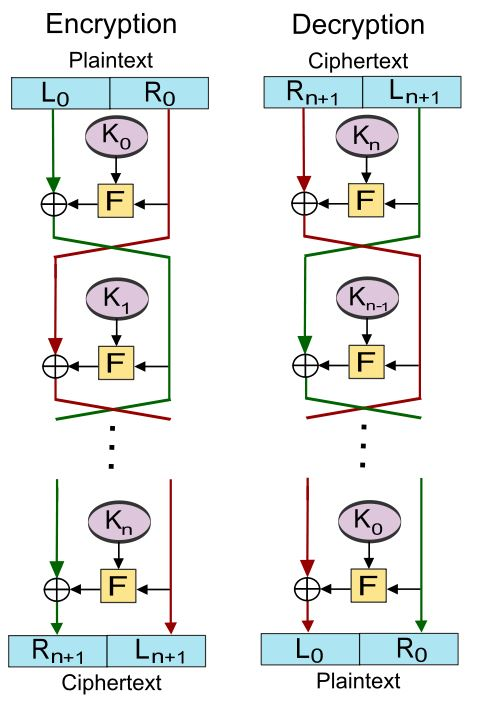
\includegraphics[width=\textwidth]{Feistel}
%            \centering
%            \caption{Basic Feistel network.}
%            \label{Feistel}
%    \end{subfigure}
%    \begin{subfigure}[H]{0.5\textwidth}
%            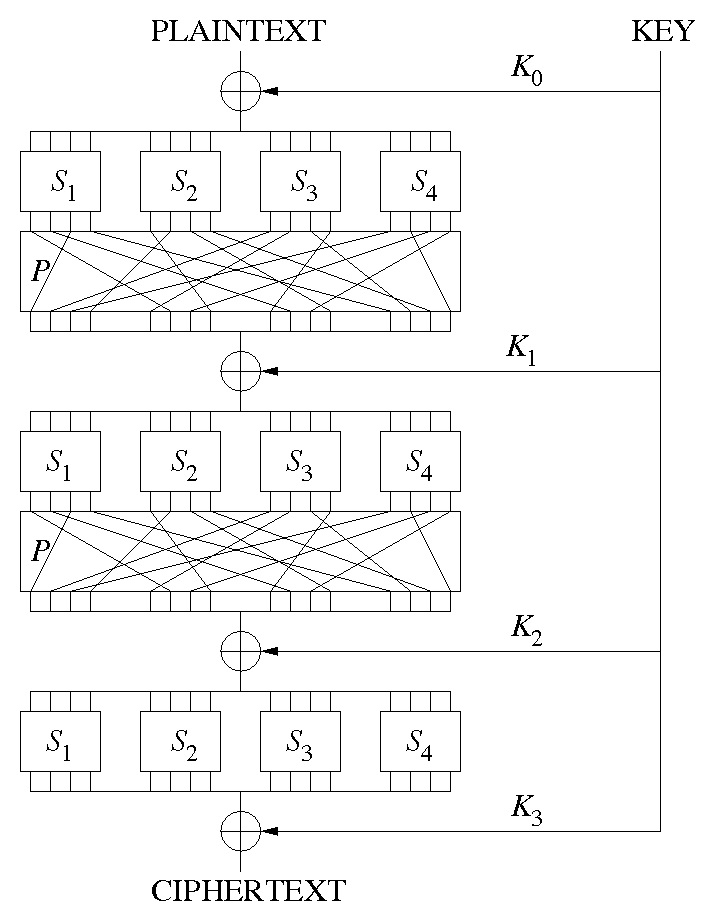
\includegraphics[width=\textwidth]{SP}
%            \centering
%            \caption{Basic Substitution Permutation network.}
%            \label{SP}
%    \end{subfigure}
%    \end{figure}

    \begin{equation}
    \label{F_L_ENC}
    L_{i+1} = R_i
    \end{equation}
    \begin{equation}
    \label{F_R_ENC}
    R_{i+1} = L_i \oplus F(R_i, K_i)
    \end{equation}
    \begin{equation}
    \label{F_L_DEC}
    R_i = R_{i+1}
    \end{equation}
    \begin{equation}
    \label{F_R_DEC}
    L_i = R_{i+1} \oplus F(L_{i+1}, K_i)
    \end{equation}
    
    On the other hand, Substitution Permutation networks operate on the whole plaintext block using S-boxes for substitution and P-boxes for permutation. Individually, these operations aren't particularly strong as a S-box and a P-box can be thought of as simple substitution and transposition ciphers respectively. However, when combined in a SP network over multiple rounds the security can be very strong due to Shannon's confusion, provided by the S-boxes, and diffusion, P-boxes, properties being satisfied\cite{Shannon1949}. The S-boxes usually take in a certain number of bits and outputs the same number of bits but of a different value. P-boxes are then used to spread the bits around such that the output of the S-boxes are used by as many S-boxes in the next round. After the S-boxes and P-boxes and before the next round occurs the block is XORed with the round key so the round equation is \autoref{SP_ENC}. Decryption, \autoref{SP_DEC} is achieved using inverted S-boxes and P-boxes and the round keys in reverse order which means that different hardware or operations are needed.
    
    \begin{equation}
    \label{SP_ENC}
    B_{i+1} = F(B_i) \oplus K_i
    \end{equation}
    \begin{equation}
    \label{SP_DEC}
    L_i = R_{i+1} \oplus F(L_{i+1}, K_i)B_i = F'(B_{i+1}) \oplus K_i
    \end{equation}
    
    \textcolor{red}{CHANGE/IMPROVE BELOW} 
    
    Stream ciphers were initially designed to approximate the One Time Pad (OTP) cipher that was proved to be completely unbreakable by Claude Shannon\textcolor{red}{[insert reference]}. The OTP works by combining each digit of the plaintext with a completely random keystream. The stream ciphers work by generating a pseudo-random keystream to combine with the plaintext\cite{Robshaw1995}. Because the keystream is pseudo-random and not completely random a stream cipher is breakable. The keystream is created by a pseudo-random number generated with a cryptographic key used as a seed.   
    
    There are also some modes of operation for block ciphers, in \cite{Dworkin2001}, that provide better security by using feedback of the ciphertext to the next block. Some of these modes of operation also allow block ciphers to behave similar to stream ciphers as they encrypt an initialization vector with the key and the resulting ciphertext can be combined with the plaintext.
    
    \subsection{Decisions}
    \label{section:cryp_decisions}
    
    \textcolor{orange}{POSSIBLY CHANGE/IMPROVE BELOW}
    
    Due to the fact that asymmetric key algorithms are hard to solve they require complex hardware or software to implement which is undesirable for this project. Also, with the exception of ECC the key sizes needed for the security can be very large so with the limited IO pins available on FPGAs they could prove difficult to program. On the other hand, many private key algorithms are designed to be efficient in hardware especially Feistel networks as an inverted round function isn't required. While a stream cipher can be useful to encrypt serial data that will most likely be the source, the modes of operation available for block ciphers provide more flexible functionality including stream cipher modes. Therefore, the algorithm chosen for this project will most likely be a block cipher with a Feistel network.
    
    \section{Conventional Algorithms}

    \textcolor{orange}{POSSIBLY CHANGE/IMPROVE BELOW}
    
    There are many block ciphers that are considered very secure and therefore popular, they include: DES\cite{ComputerSecurityDivision1999}, AES\cite{ComputerSecurityDivision2001}, Blowfish\cite{BruceSchneier1994}.
    DES operates on a block of 64 bits for 16 rounds using a key length of 64 bits but it has an effective key length of 56 bits as 8 bits were used for parity.
    AES, an upgrade to DES, is far more secure as uses a 128 bit block and has the flexibility of using three different key lengths: 128, 192 and 256. The number of rounds that AES iterates depends on the key length with 10 rounds used for a 128 bit key, 12 for 192, and 14 for the largest key.
    Blowfish, like DES, operates on a 64 bit block and iterates for 16 rounds, but it can use a variable key length in the range 32 to 448 bits.
    
    \subsection{Standardization}
    DES, which stands for Data Encryption Standard, is one the earliest block ciphers used in the computer age and it was developed by IBM in the 1970s based on their earlier cipher Lucifer\textcolor{red}{[insert reference]}. As with Lucifer it was designed around a Feistel network but the round function used also has a SP network structure to it\textcolor{red}{[insert reference]},but the S-boxes aren't a one-to-one function but rather output 4 bits from a 6 bit input. It has the name Data Encryption Standard as it was accepted as the standard encryption algorithm by the US National Bureau of Standards (NBS), now the National Institute of Standards and Technology (NIST), in 1977 after it was altered by the National Security Agency (NSA), which caused some controversy\cite{ComputerSecurityDivision1999}.
    
    DES was used for about two decades but in the 1990s several successful attacks proved its weakness\cite{Team} so in 1997 NIST started a selection process to find its replacement. Due the controversy of the NSAs involvement and comments from the cryptography community the selection process was as transparent as possible\textcolor{red}{[insert reference]}. Many algorithms were submitted as candidates for the standard but the finalists were: MARS, RC6, Rijndael, Serpent, and Twofish\textcolor{red}{[insert reference]}. It took three years to decide on the algorithm to be set as the standard which was announced as Rijndael in 2000 and the standard was et in 2001, with the 128, 192, 256 bit keys being used in the standard\cite{ComputerSecurityDivision2001}. Unlike DES, AES uses a SP network as it is efficient, in time, in both hardware and software. The round function treats the block as a $4x4$ byte matrix and performs multiple steps on the data: sub bytes; shift rows; mix columns and add round key\textcolor{red}{[insert reference]}.
    %The sub bytes uses S-boxes with byte inputs and outputs another byte based on a lookup table.
    %The shift row step then shifts each of the rows in the matrix by the same number of bytes as the row number.
    %The mix column step is the most complicated as it involves matrix multiplication in the finite field $GF(2^8)$, but is commonly implemented in lookup tables.
    %The add round key step is the simplest as it is just XORing the block with the key generated by the key schedule.
    
    Since its standardization in 2001 AES has been used almost exclusively because its security is trusted. Because of this there are many different software and hardware implementations produced with some concentrating on side-channel attack resistance\cite{Strachacki2008} or efficient S-box implementations\cite{Gomes2016}. However, even area optimized designs like \cite{Moradi2011} use 2400 gate equivalents which is too much for lightweight applications.
    
    \subsection{Other Algorithms}
    The US standardized algorithms quickly became very popular and can be considered the unofficial global standard.
    Although, there are many other algorithms that are considered secure and are commonly used. One of these algorithms, TripleDES, is actually based around DES which increases the security by encrypting the plaintext three times with separate keys making the effective key length of 168 bits.
    These algorithms might be used because there is still some distrust of the NSAs involvement in the algorithms and they are more open source. This is the case of the Blowfish algorithm as it is unpatented and can therefore be used in any product without legal consequence.
    
    Blowfish was designed by Bruce Schneier in the early 1990s as he, and many others, noticed the insecurity of DES particularly with the 56 bit key length making a brute force attack more plausible\cite{BruceSchneier1994}. The design of the algorithm is based around a Feistel network with, similar to DES, the round function using S-boxes. The sub keys and S-box lookup tables are generated using the hexadecimal digits of pi which are provided by the designers\textcolor{red}{[insert reference]}. As with AES there are many FPGA and ASIC implementations of the Blowfish algorithm, \cite{Chatterjee2014} and \cite{Prasetyo2014}, but they require too many FPGA resources to be considered for the lightweight nature of this project.
    
    \subsection{Decisions}
    Due to the conventional algorithms not being explicitly designed for hardware and definitely not for lightweight applications they are not appropriate for this project. Although, they are useful for comparison with the lightweight algorithms in \autoref{section:light} in terms of security and throughput.
    
    \section{Lightweight Algorithms}
    \label{section:light}
    After deciding that the conventional algorithms might not be suitable for the low power devices targeted by this project, some more lightweight algorithms were found including: PRESENT\cite{Bogdanov2007}, PRINCE\cite{Borghoff2012} and the SIMON and SPECK algorithms\cite{Beaulieu2013}. However, as IoT is an emerging technology and is the main reason for lightweight cryptography there isn't a standard set by NIST, but the process has begun in \cite{Mckay}. These algorithms are considered lightweight because they make sacrifices in and security or throughput, or both, to achieve small area and low power designs.
    
    \subsection{SIMON \& SPECK}
    The SIMON and SPECK family of algorithms are the lightweight techniques proposed by the NSA that were designed to perform well in both software and hardware while still being secure; and to be flexible in terms of block and key size, listed in \autoref{table:S+S}. The algorithms are similar but SIMON was optimised for hardware implementations and SPECK for software. As with AES the number of rounds iterated depends on the key size but as the block size varies as well it also has an effect as shown in \autoref{table:S+S}.
    The structure of both algorithms is a Feistel network and thus it works on words of $n$ bits, where $2n$ is the block size, and with a key of $mn$ bits. This lends it self to the naming format of SIMON or SPECK $2n/mn$, which means, for example, SIMON48/72 has a word size of 24 and uses 3 words for the key\textcolor{red}{[insert reference]}.
    
        \begin{table}[H]
        \centering
        \begin{tabular}{||c|c|c|c|c|c||}
            \hline \hline
            Block Size & Key Size & $n$ & $m$ & SIMON Rounds & SPECK Rounds \\
            \hline \hline
            32 & 64 & 16 & 4 & 32 & 22 \\
            \hline
            48 & 72 & 24 & 3 & 36 & 22 \\
            48 & 96 & 24 & 4 & 36 & 23 \\
            \hline
            64 & 96 & 32 & 3 & 42 & 26 \\
            64 & 128 & 32 & 4 & 44 & 27 \\
            \hline
            96 & 96 & 48 & 2 & 52 & 28 \\
            96 & 144 & 48 & 3 & 54 & 29 \\
            \hline
            128 & 128 & 64 & 2 & 68 & 32 \\
            128 & 192 & 64 & 3 & 69 & 33 \\
            128 & 256 & 64 & 4 & 72 & 34 \\
            \hline \hline
        \end{tabular}
        \caption{A table of the modes of operation for the SIMON \& SPECK Algorithms. Adapted from \cite{Beaulieu2015}.}
        \label{table:S+S}
        \end{table}    
    
    %\textcolor{cyan}{[Insert FPGA implementations of SIMON \& SPECK]}
    Even though they are relatively new algorithms there are still a few FPGA implementations available for review, including \cite{Aysu2014} and \cite{Shahverdi2015} as well as those provided in \cite{Beaulieu2013}. These all show that very small designs are possible with even the 128/256 versions fitting below the 2000 GE limit.
    
    \subsection{Other Algorithms}
    The PRESENT cipher is another option for lightweight cryptography as it achieves a 1570 GE FPGA design with a 80 bit working on a 64 bit block. there is also an version that uses 128 bit key. The design of the cipher is based around a SP network, \autoref{Feistel}, with 64 bit subkeys.
    
    PRINCE is a lightweight cipher that can encrypt data in one clock cycle with an unrolled SP network, as SP networks require less rounds than a F network. The steps include S-boxes and a matrix layer as well as the XORing of the round key and a round constant. Due to the unrolled nature of the algorithm the FPGA implementations are mainly combinational so the register count is lower than other algorithms.
    
    \subsection{Decisions}
    Based on the research explored in \autoref{chapter:research} I chose the SIMON and SPECK algorithms from the NSA, mainly because of their flexibility in security levels, with different key lengths, that could be applied to the different devices explored in \autoref{section:IoT}. This means that multiple algorithms don't need to be developed and I could concentrate on making my code as efficient as possible. When compared in terms of power consumption the SIMON64/96 version in \cite{Banik2015} also shows lower power consumption than the other algorithms explored. Also, while both PRESENT and PRINCE meet the lightweight specification they are also SP networks and in \autoref{section:cryp_decisions} it was decided that a Feistel network is preferable.
    
    After deciding on the SIMON and SPECK family I explored how each version works in order to make a more informed decision on which to work with in this project. As SIMON was designed primarily for hardware it only makes use of XOR ($\oplus$), AND ($\&$) and circular rotate operations ($R^j[x]$) on the $n$ bit wide words. For the rotate operation the word $x$ is rotated by $j$ bits to the left or right if $j$ is negative. The encryption and decryption functions take the Feistel network form described in \autoref{Feistel} with the round function \autoref{SIMON_round}.
    
    \begin{equation}
    \label{SIMON_round}
    F(x) = (R^1[x]\&R^8[x]) \oplus R^2[x]
    \end{equation}
    
    SPECK on the other hand, being optimised for software implementations uses XOR ($\oplus$), modulo $2^n$ addition ($+$) and circular rotate operations ($R^j[x]$), with the circular rotate being equivalent to what is used in SIMON. The encryption and decryption functions take a slightly different form to the basic Feistel network, \autoref{Feistel}, and are shown in \autoref{SPECK_L_round} and \ref{SPECK_R_round} where $\alpha = 7$ and $\beta = 2$ if $n = 16$, but $\alpha = 8$ and $\beta = 3$ otherwise.
    
    \begin{equation}
    \label{SPECK_L_round}
    L_{i+1} = (R^{-\alpha}[L_i] + R_i) \oplus K_i
    \end{equation}
    \begin{equation}
    \label{SPECK_R_round}
    R_{i+1} = R^{\beta}[R_i] \oplus (R^{-\alpha}[L_i] + R_i) \oplus K_i = R^{\beta}[R_i] \oplus L_{i+1}
    \end{equation}
    As the aim of this project is to compare how an algorithm performs in hardware and software SIMON was chosen even though SPECK shows almost as good performance in hardware and much better in software. 
    
    \chapter{Previous Work \& Initial Design Approaches}
    \label{chapter:INITIAL}
    
    \chapter{Final Design Approach}
    \label{chapter:FINAL}
    
    \chapter{Experiments \& Results}
    \label{chapter:RESULT}
    
    \chapter{Conclusion \& Future Work}
    \label{chapter:CONC}
    
    \bibliographystyle{IEEEtran}
    \bibliography{Report}
    \addcontentsline{toc}{chapter}{Bibliography}
    
    \appendix    
    
    \chapter{New Appendix}
    
\end{document}